Das Ziel von Gasdetektoren ist die Messung bzw. Zählung der $e^-$-Ion-Paare. Ein Problem dabei
ergibt sich aus der Reduktion der Anzahl der $e^-$-Ion-Paare durch Rekombination und
Elektronanlagerung.
\\
Die Rekombination erfolgt nach dem Schema

\[A^+ + e^- \longrightarrow A + h\nu \]
\[A^+ + B^- \longrightarrow AB + h\nu  \]

Die Rekombinationsrate $dn$ hängt von den Konzentrationen des positiven ($n^+$) und negativen
($n^-$) Teilchen ab:

\[dn= \text{const}\cdot n^+ n^- \mathrm{d}t \]

Wenn $n^+=n^-\equiv n$ ist, dann folgt

\[n(t) = \frac{n_0}{1+\text{const}\cdot n_0\cdot t}  \]

\begin{figure}[H]
	\centering
	
\includegraphics[width=0.5\textwidth]{dummy.jpg}
\end{figure}

Eine Aufgabe bei der Konstruktion einer Detektors ist also, eine möglichst schnelle Trennung von
positiven und negativen Ladungen aus der Ionisation herbeizuführen.
\\
Bestimmte Atome bzw. Moleküle haben eine große Elektronenaffinität, beispielsweise wenn nur wenige
Elektronen zum Abschluss einer Schale fehlen. Diese stellen regelrechte "`Fallen"' für
freie Elektronen im Gas dar. Beispiele sind O$_2$, Cl$_2$, NH$_3$, H$_2$O, CCl$_4$ oder SF$_6$.
\\
Andere Gase (N$_2$, H$_2$, CH$_4$) haben vernachlässigbare oder sogar negative
Elektronenaffinität (Edelgase). Zudem hängt die Anlagerungswahrscheinlichkeit von der $e^-$-Energie
ab.

\begin{figure}[H]
	\centering
	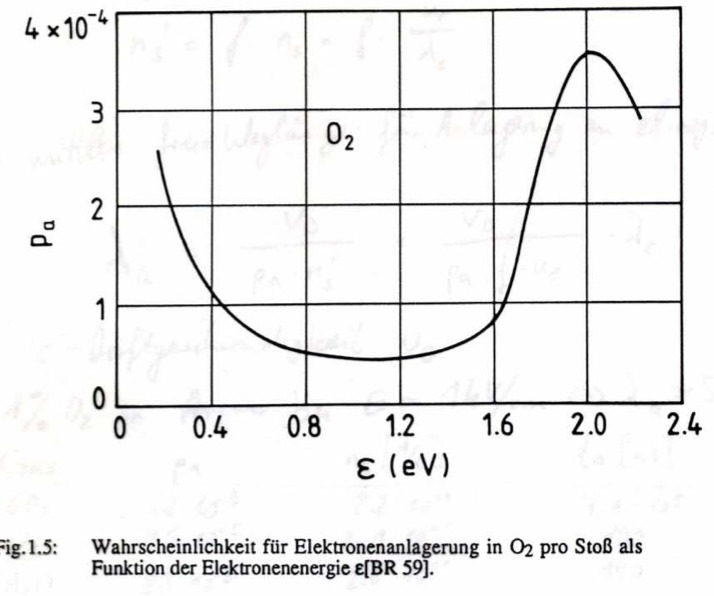
\includegraphics[width=0.5\textwidth]{Fig-03-05.jpg}
\end{figure}

Aus der thermischen Geschwindigkeit der Elektronen 

\[u_e = \sqrt{\frac{8kT}{\pi m}}  \]

und der mittleren freien Weglänge der Elektronen $\lambda_e \approx 4\cdot \lambda_{\text{Ion}}$
ergibt sich die Anzahl der Stöße pro Zeitintervall $n_S$:

\[ n_S = \frac{u_e}{\lambda_e}  \]

und daraus die Anlagerungswahrscheinlichkeit $p_a$ pro Stoß die mittlere Zeit bis zur Anlagerung

\[t_a=\frac{1}{p_a\cdot n_S}  .\]

Wenn elektronegative Moleküle mit dem Anteil f im Gas vorliegen, reduziert sich die Stoßrate zu

\[n_S' = f\cdot n_S = f\cdot \frac{u_e}{\lambda_e} \]

und für eine Driftgeschwindigkeit $v_D$ der Elektronen folgt als mittlere Weglänge bis zu Anlagerung

\[\lambda_a = \frac{v_D}{p_a\cdot n_S'}=\frac{1}{p_a\cdot f}\cdot \frac{v_D}{u_e}\cdot \lambda_e  
.\]

Beispiel: 1\% O$_2$ in Argon ergibt bei einer Driftfeldstärke von $E=1\,$keV/cm etwa
$\lambda_a\approx5\,$cm, was einen Verlust von Elektronen bei großen Driftdistanzen bedeutet.
